\documentclass[tikz]{standalone}

\tikzset{declare function={f(\x)=0.25*(\x-2.5)^3-0.75*\x+5);}}
\newcommand{\myfunction}[2]
{
  \begin{scope}[shift={(#1,0)}]
  \draw[-latex] (-0.5,0) -- (5,0) node[below] {$x$};
  \draw[-latex] (0,-0.5) -- (0,5) node[left]  {$y$};
  \draw[thick,cyan] plot[domain=0.5:4.5,samples=41] (\x,{f(\x)});
  \node at (3.25,3.5) {$y=f(x)$};
  \foreach\i in {0,1,2,3,...,8}
  {
    \pgfmathsetmacro\j{0.5*\i+0.5}
    \coordinate (x\i) at (\j,0);
    \coordinate (y\i) at (\j,{f(\j)});
  }
  \foreach\i in {0,1,2}
    \node[below]        at (x\i) {$x_\i$};
  \node[below]          at (x7) {$x_{n-1}$};
  \node[below]          at (x8) {$x_n$};
  \node[yshift=-0.75cm] at (x0) {\strut$a$};
  \node[yshift=-0.75cm] at (x8) {\strut$b$};
  \node[yshift=-1cm]    at (x4) {#2};
  \end{scope}
}

\begin{document}
    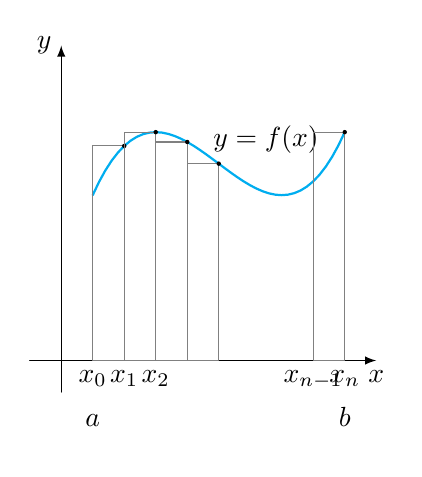
\begin{tikzpicture}[line join=round,line cap=round,scale=0.8]
        \myfunction{6}{}
        \foreach\i in {0,1,2,3,7}
        {
          \pgfmathtruncatemacro\j{\i+1}
          \draw[gray] (x\i) rectangle (y\j);
          \fill (y\j) circle (1pt);
        } 
    \end{tikzpicture}
\end{document}